\documentclass[12pt]{article}

%Begin----------------------------------------------------------------------------------------------------------------------------------------
%---------------------------------------------------------------------------------------------------------------------------------------------


%Package import and Config of Packages
%\usepackage[utf8]{inputenc}%\usepackage{tikz}#
\usepackage{lmodern}
\usepackage{setspace}
\usepackage{lastpage}
\usepackage{pgfplots} % Fuer Plots
\usepackage{pgfplotstable}
\usepackage{pgfkeys} 
\pgfplotsset{compat = newest}
\usepackage{tikz} % Generell gutes Packet
\usepackage{csvsimple} % Zum CSV auslesen
\usepackage{fancyhdr}
\usepackage{tcolorbox}


\usepackage[ngerman]{babel}
\usepackage{datetime}
\newdateformat{myformat}{\THEDAY{ten }\monthname[\THEMONTH], \THEYEAR}


\usepackage{subfig}
\usepackage{pdfpages}
\usepackage{subfiles}
\usepackage{titlesec}
\usepackage[pdfborder={0 0 0}]{hyperref}
\usepackage{pdfpages}
\usepackage{verbatim}
\usepackage{geometry}
\geometry{left=20mm, right=20mm, bottom=20mm}

\usepackage{graphicx}
\graphicspath{{../Bilder/}{Bilder/}}

\usepackage{xcolor}
\usepackage{listings}
%End------------------------------------------------------------------------------------------------------------------------------------------
%---------------------------------------------------------------------------------------------------------------------------------------------
%Package import and Config of Packages

%Begin----------------------------------------------------------------------------------------------------------------------------------------
%---------------------------------------------------------------------------------------------------------------------------------------------
%List Configuration for Coding
\usepackage{listings} % Generell Code-Boxen
\usepackage{xcolor} % Fuer extra Farben mit color{}

\colorlet{punct}{red!60!black}
\definecolor{background}{HTML}{EEEEEE}
\definecolor{delim}{RGB}{20,105,176}
\colorlet{numb}{magenta!60!black}

\definecolor{mGreen}{rgb}{0,0.6,0}
\definecolor{mGray}{rgb}{0.5,0.5,0.5}
\definecolor{mPurple}{rgb}{0.58,0,0.82}
\definecolor{backgroundColour}{rgb}{255,255,255}

\lstdefinestyle{StyleC}
{
    frameround=tttt,
    numbers=left,
    backgroundcolor=\color{backgroundColour},
    belowcaptionskip=1\baselineskip,
    breaklines=true,
    xleftmargin=\parindent,
    language=C,
    frame = single,
    showstringspaces=false,
    basicstyle=\footnotesize\ttfamily,
    keywordstyle=\bfseries\color{magenta},
    commentstyle=\color{mGreen},
    identifierstyle=\color{blue},
    stringstyle=\color{orange},
} 

%End------------------------------------------------------------------------------------------------------------------------------------------
%---------------------------------------------------------------------------------------------------------------------------------------------
%List Configuration for Coding


%Begin----------------------------------------------------------------------------------------------------------------------------------------
%---------------------------------------------------------------------------------------------------------------------------------------------
%More Subsections Configuration
\titleclass{\subsubsubsection}{straight}[\subsection]
\newcounter{subsubsubsection}[subsubsection]
\renewcommand\thesubsubsubsection{\thesubsubsection.\arabic{subsubsubsection}}
\renewcommand\theparagraph{\thesubsubsubsection.\arabic{paragraph}} % optional; useful if paragraphs are to be numbered
\titleformat{\subsubsubsection}
  {\normalfont\normalsize\bfseries}{\thesubsubsubsection}{1em}{}
\titlespacing*{\subsubsubsection}
{0pt}{3.25ex plus 1ex minus .2ex}{1.5ex plus .2ex}


\titleclass{\subsubsubsubsection}{straight}[\subsection]
\newcounter{subsubsubsubsection}[subsubsubsection]
\renewcommand\thesubsubsubsubsection{\thesubsubsubsection.\arabic{subsubsubsubsection}}
\titleformat{\subsubsubsubsection}
  {\normalfont\normalsize\bfseries}{\thesubsubsubsubsection}{1em}{}
\titlespacing*{\subsubsubsubsection}
{0pt}{3.25ex plus 1ex minus .2ex}{1.5ex plus .2ex}

\makeatletter
\renewcommand\paragraph{\@startsection{paragraph}{5}{\z@}%
  {3.25ex \@plus1ex \@minus.2ex}%
  {-1em}%
  {\normalfont\normalsize\bfseries}}
\renewcommand\subparagraph{\@startsection{subparagraph}{6}{\parindent}%
  {3.25ex \@plus1ex \@minus .2ex}%
  {-1em}%
  {\normalfont\normalsize\bfseries}}
\def\toclevel@subsubsubsection{4}
\def\toclevel@paragraph{5}
\def\toclevel@paragraph{6}
\def\l@subsubsubsection{\@dottedtocline{4}{7em}{4em}}
\def\l@subsubsubsubsection{\@dottedtocline{5}{8em}{5em}}
\def\l@paragraph{\@dottedtocline{5}{10em}{5em}}
\def\l@subparagraph{\@dottedtocline{6}{14em}{6em}}
\makeatother

\setcounter{secnumdepth}{5}
\setcounter{tocdepth}{5}

%End------------------------------------------------------------------------------------------------------------------------------------------
%---------------------------------------------------------------------------------------------------------------------------------------------
%More Subsections Configuration


\pagestyle{fancy}
\fancyhf{}


%Begin----------------------------------------------------------------------------------------------------------------------------------------
%---------------------------------------------------------------------------------------------------------------------------------------------
%TitelSeite
\title{
  \vspace{-2cm}
  \centering
  
\includegraphics[width=\linewidth]{htl-logo.jpg}\\
  noindent\rule{\linewidth}{1pt}\\
  \vspace{50px}
  \Huge\textbf{\textsc{DIC-serial\_crypto}}
  \normalsize 
}
\author{Fabio~Plunser}
\date{\today}
\rhead{\hspace{5px}
\includegraphics[scale=0.09]{htl-logo.jpg}}
\lhead{DIC-serial\_crypt}
\rfoot{Page~\thepage ~of~\pageref{LastPage}}
\lfoot{PlunserFabio}
\renewcommand{\headrulewidth}{1pt}
\renewcommand{\footrulewidth}{1pt}

\newcommand{\anfuehrung}[1]{\glqq #1\grqq{}}

\begin{document}
\pagenumbering{gobble}

\begin{titlepage}
  \maketitle
  \begin{figure}[!htb]
    \centering
    
\includegraphics[scale=1]{zephyr-logo.png}
    \label{zephyr-logo}
  \end{figure}

\end{titlepage}

%End------------------------------------------------------------------------------------------------------------------------------------------
%---------------------------------------------------------------------------------------------------------------------------------------------
%TitelSeite

%Begin----------------------------------------------------------------------------------------------------------------------------------------
%---------------------------------------------------------------------------------------------------------------------------------------------
%Inhaltsverzeichnis
\pagebreak
\thispagestyle{empty}
\renewcommand\contentsname{Inhaltsverzeichnis}
\tableofcontents	
\pagenumbering{gobble}

%End------------------------------------------------------------------------------------------------------------------------------------------
%---------------------------------------------------------------------------------------------------------------------------------------------
%Inhaltsverzeichnis

%Begin----------------------------------------------------------------------------------------------------------------------------------------
%---------------------------------------------------------------------------------------------------------------------------------------------
%Abbildungsverzeichnis
\thispagestyle{empty}
\renewcommand\listfigurename{Abbildungsverzeichnis}
\listoffigures
%End------------------------------------------------------------------------------------------------------------------------------------------
%---------------------------------------------------------------------------------------------------------------------------------------------
%Abbildungsverzeichnis
\renewcommand\lstlistlistingname{Code}
\lstlistoflistings

%Begin----------------------------------------------------------------------------------------------------------------------------------------
%---------------------------------------------------------------------------------------------------------------------------------------------
%Codeverzeichnis
% \renewcommand\lstlistlistingname{Codeverzeichnis}
% \lstlistoflistings
\pagebreak
\pagenumbering{arabic}

%End------------------------------------------------------------------------------------------------------------------------------------------
%---------------------------------------------------------------------------------------------------------------------------------------------
%Codeverzeichnis



%Begin----------------------------------------------------------------------------------------------------------------------------------------
%---------------------------------------------------------------------------------------------------------------------------------------------
%Main
\newpage
\section{Aufgabenstellung}
    Die Aufgabe ist es auf dem STM32F030F4 Chip die UART3 so zu programmieren, dass sie den Wert eines eingebauten ADC per interrupt ausgibt.\\
    Die richtige Aufgabe ist es die STM32F030F4 UART3 zu programmieren dass sie wenn sie ein zeichen erhält 10 Bytes zurückschickt. \\
    Da dieses spezielle Package des STM32 keine UART3 besitzt ist die Aufgabenstellung so nicht möglich somit wird einfach die vorhandene UART1 Schnittstelle verwendet.\\
    Der STM UART Ausgang wird mit einem MAX485 auf RS485 übersetzt.\\
    UART einstellungen:\\
    Baudrate: 38400 mit ODD parity\\\\
    
    \noindent Dieser Arbeitsauftrag kann in dieser GIT-Repo verfolgt werden: \url{https://github.com/FabioPlunser/DIC-Lezuo}
    


\newpage
\section{Theorie und Vorwissen}
\subsection{Zephyr}
    Zephyr ist ein Open-Source-Echtzeitbetriebssystem welches von der Linux Foundation.\footnote{Quelle: \url{https://de.wikipedia.org/wiki/Zephyr_(Betriebssystem)}}
    Ein Echtzeitbetriebssystem, real-time operating system \textbf{RTOS} ist ein Betriebssystem, das Echtzeit-Anforderungen erfüllen kann. 
    Das bedeutet, dass Anfragen eines Anwendungsprogramms innerhalb einer Voraus bestimmbaren Zeit gesichert verarbeitet werden.\footnote{Quelle: \url{https://de.wikipedia.org/wiki/Echtzeitbetriebssystem}}
    \\
    Zephyr wurde mit dem \href{https://docs.zephyrproject.org/latest/getting_started/index.html}{Getting-Started-GUID} Linux Subsystem von Windows installiert. 
    Um ein Zephyr Projekt zu kompilieren wird Zephyr eigenes \textbf{West}\footnote{\url{https://docs.zephyrproject.org/2.4.0/guides/west/index.html}} verwendet.\\
    \textbf{West} ist ein Kompilierungs-Tool von Zephyr. Es verwendet Ninja und CMake um das Projekt zu kompilieren. 
    West wird folgendermaßen verwendet, um ein Projekt zu kompilieren: 
    \begin{lstlisting}[style=StyleC, captionpos=b, caption=West Beispiel, label=West Beispiel]
west build -p auto -b nativ_posix_64 
    \end{lstlisting}

\newpage
    \subsubsection{west}
        \subsubsubsection{West als Repo Verwalter}
            West ist ein Command-line tool von Zephyr. Es wird unabhängig von Zephyr installiert und wird zur Kompilierung und Flashen verwendet. 
            Das Problem das bei solchen Projekten entsteht ist, dass es sich aus mehreren GIT Repositories mit unterschiedlichen Versionen zusammen setzen kann, somit
            muss dafür gesorgt werden, dass alle GIT Repositories, mit der korrekter Version im korrekten pfad sich befinden. 
            Diese werden im sogenannten \textit{west manifest} \textbf{west.yaml} festgelegt.\footnote{\url{https://docs.zephyrproject.org/latest/guides/west/index.html}}
            \begin{lstlisting}[style=StylePython, captionpos=b, caption=west.yaml]
manifest:
defaults:
    remote: upstream

remotes:
    - name: upstream
    url-base: https://github.com/zephyrproject-rtos

#
# Please add items below based on alphabetical order
projects:
    - name: cmsis
    revision: c3bd2094f92d574377f7af2aec147ae181aa5f8e
    repo-path: mcuboot
    path: modules/tee/tfm-mcuboot
    revision: 1.7.0-rc1
    ...
self:
    path: zephyr
    west-commands: scripts/west-commands.yml    
            \end{lstlisting} 
            Um einen Ordner zu initialisieren wird \textbf{west init} und zum downloaden der Daten \textbf{west update} verwendet.\footnote{\url{https://github.com/zephyrproject-rtos/west}}
        \subsubsubsection{West als Compiler}
            West ist der Haupt-Compiler von Zephyr, west ruft cmake, ninja oder make im Hintergrund auf um erfolgreich zu Kompilieren. 
            Im Hintergrund wird hauptsächlich ninja verwendet.\footnote{\url{https://docs.zephyrproject.org/latest/application/index.html?highlight=ninja}}


\newpage
    \subsubsection{ninja}
        Ninja ist ein kleines build System mit Fokus auf Geschwindigkeit. 
        Es ist in assembler geschrieben und ist so designend, dass die Input files von einem höheren Build-System erstellt werden und das es so schnell wie möglich builded. 
        Das Problem, das die Ninja entwickler mit GNU Make hatten, ist das es durch die Higher-Level Programmiersprache für große Projekte recht viel Zeit benötigt. 
        Durch die Implementierung in Assembler steigt die Geschwindigkeit stark und ist somit sehr gut für große Projekte geeignet, jedoch steigt auch die Komplexität. 

    \subsubsection{KConfig}
    \textbf{Kernel Configuration File}\footnote{\url{https://docs.zephyrproject.org/latest/application/index.html?\#application-kconfig}}ist die \textcolor{red}{prj.conf} Datei in einem 
    Zephyr Projekt. In diesem werden besstimmte Konfigurationen, Funktionen und \anfuehrung{Geräte}, wie z.b. \textit{CONFIG\_SERIAL=y} aktiviert. 
    Das Ziel ist es alle im Kernel beinhaltete Funktionen, Applikations spezifisch, zur Verfügung zu stellen, ohne den Source Code ändern zu müssen. 
    Somit können Funktionen und Schnittstellen einfach aktiviert werden. 
    Welche Schnittstellen für ein board aktiviert werden können, kann im Device Tree gefunden werden. 

\newpage
    \subsubsection{Device Tree}
    Der Device Tree\footnote{\url{https://docs.zephyrproject.org/latest/guides/dts/intro.html}\\\url{https://docs.zephyrproject.org/latest/reference/devicetree/index.html\#devicetree}} ist 
    in einem Zephyr Projekt eine Datei mit der Endung \textbf{.dts} dort stehen alle für das ausgewählte Board verfügbare Geräte drinnen.
    Im Fall des nativ\_posix\_64 sieht dieses folgendermaßen aus. 
    \begin{lstlisting}[style=StyleC, captionpos=b, caption=West Beispiel, label=West Beispiel]
/dts-v1/;

/ {
    #address-cells = < 0x1 >;
    #size-cells = < 0x1 >;
    model = "Native POSIX Board";
    compatible = "zephyr,posix";
    chosen {
        zephyr,console = &uart0;
        zephyr,shell-uart = &uart0;
        zephyr,uart-mcumgr = &uart0;
        zephyr,flash = &flash0;
        zephyr,entropy = &rng;
        zephyr,flash-controller = &flashcontroller0;
        zephyr,ec-host-interface = &hcp;
    };
    aliases {
        eeprom-0 = &eeprom0;
        i2c-0 = &i2c0;
        spi-0 = &spi0;
        led0 = &led0;
    };
    leds {
        compatible = "gpio-leds";
        led0: led_0 {
            gpios = < &gpio0 0x0 0x0 >;
            label = "Green LED";
        };
    };

    ...

    };
    uart0: uart {
        status = "okay";
        compatible = "zephyr,native-posix-uart";
        label = "UART_0";
        current-speed = < 0x0 >;
    };
    
    ...

};    
    \end{lstlisting}


\newpage
    \subsubsection{Tinycrypt}
    Die TinyCrypt-Bibliothek bietet eine Implementierung für eingeschränkte Geräte von minimalen Standard-Kryptographie-Grundelementen.
    Di Bibliothek ist von Intel\footnote{\url{https://github.com/intel/tinycrypt}} und wurde in zephyr mit der implementiert.\footnote{\url{https://docs.zephyrproject.org/2.3.0/guides/crypto/tinycrypt.html?highlight=tinycrypt}} 
    Innerhalb von Zephyr können die eignenen Crypto API Befehle oder die direkten TinyCrypt Befehle verwendet werden. 

     
\subsection{Linux Pseudoterminal}
Ein Pseudoterminal ist ein Dienst der eine bidirektionale Pipe, aufbaut. Sie werden verwendet um ein physisches Terminal zu emulieren. 
Im Fall von Zephyr mit dem nativ\_posx Board wird ein Pseudoterminal verwendet um mit dem Baord zu kommunizieren. Der Pfad dieses Terminals ist /dev/pts/.
\subsection{Threads}
Innerhalb eines Betriebssystems werden Applikationen und Abläufe als Prozesse realisiert. Prozesse werden vom Schedular verwaltet. Um nun die Abarbeitung dieser Prozesse zu 
beschleunigen, besteht ein ein Prozess aus mehreren parallel laufenden Threads. Diese Threads beinhalten einen Teil des Codes des Prozesses, dadurch können große Probleme entstehen. 
Es muss sichergestellt werden, dass Threads nie auf die gleichen Variablen/Ressourcen zugreifen, da ansonsten \textit{race-Conditions} entstehen. 
\begin{figure}[!htb]
    \centering
    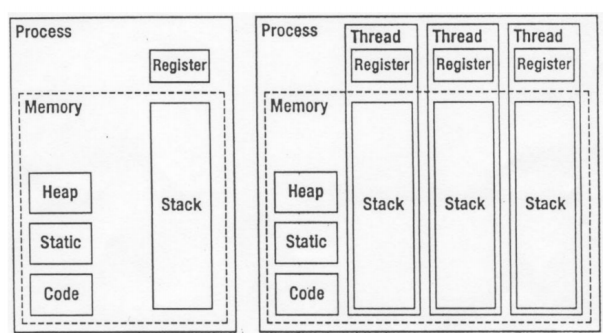
\includegraphics[width=0.65\linewidth]{Process-Threads.png}
    \caption{Process-Threads}
    \label{caption:Process-Threads}
\end{figure}

\newpage
\subsection{Message-Queue}
Eine Message-Queue ist ein besonderer Buffer, ein FIFO-Buffer (First-In-First-Out-Buffer). Das bedeutet, es werden Nachrichten in einer Reihe in den Buffer geschrieben und es kann nur die
erste Nachricht in der Reihe herausgenommen werden, dabei wird diese nachricht im Buffer gelöscht und die nächste Nachricht rückt nach. 
Solche Message-Queues werden verwendet, um zwischen Threads die Daten korrekt auszutauschen. Da eine Nachricht beim auslesen gelöscht wird, können nicht mehrere Threads gleichzeitig auf 
die Nachricht zugreifen. 
\begin{figure}[!ht]
    \centering
    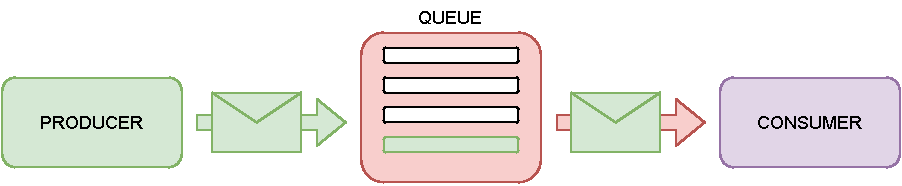
\includegraphics[width=\linewidth]{Message-Queue.pdf}
    \caption{Message-Queue-Darstellung}
    \label{fig:Message-Queue-Darstellung}
\end{figure}
\newpage
\section{Programm Umsetzung}
Das Programm wurde wie angegeben in 4 Threads eingeteilt.
\begin{itemize}
    \item Main-Thread
    \begin{itemize}
        \item Initialisierung der anderen Threads
        \item UART und Crypto Device Initialisierung 
        \item Validate Hardware Compatibility 
        \item alle 5 Sekunden ein Lebenszeichen von sich geben. 
    \end{itemize} 
    \item UART-IN-Thread
    \begin{itemize}
        \item Einlesen der UART 
        \item Statemachine Implementierung
    \end{itemize}
    \item UART-OUT-Thread
    \begin{itemize}
        \item Ausgabe der in die Queue geschriebenen Messages
    \end{itemize}
    \item PROCESS-Thread
    \begin{itemize}
        \item Verwaltung der Entschlüsselung 
    \end{itemize}
\end{itemize}
\subsection{Blockschaltbild}
\begin{figure}[!ht]
    \centering
    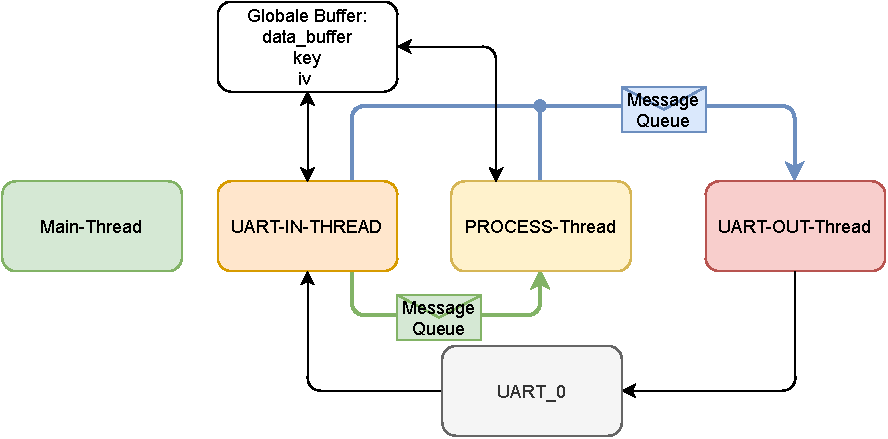
\includegraphics[width=\linewidth]{Blockschaltbild.pdf}
    \caption{Blockschaltbild}
    \label{fig:Blockschaltbild}
\end{figure}




\newpage
\subsection{Projekt Konfiguration}
Sodass, das nativ\_posix Board die benötigten Geräte verwenden kann müssen dieser in der \textbf{prj.conf} Datei aktivieren werden. 
\begin{lstlisting}[style=StyleC, captionpos=b, caption=prj.conf, label=pjr.conf]
#Configure Serial-Connection
CONFIG_SERIAL=y
CONFIG_UART_NATIVE_POSIX=y
CONFIG_NATIVE_UART_0_ON_OWN_PTY=y

#Configure Crypto
CONFIG_TINYCRYPT=y
CONFIG_TINYCRYPT_AES=y
CONFIG_TINYCRYPT_AES_CBC=y
CONFIG_CRYPTO=y
CONFIG_CRYPTO_TINYCRYPT_SHIM=y
\end{lstlisting}

\subsection{Initialisierung}
Es müssen:
\begin{itemize}
    \item Message-Queue 
    \item UART\_0 
    \item Verschlüsselung 
    \item Threads
\end{itemize}
initialisiert werden. 
    \subsubsection{Message-Queue}
        Wie in der Zephyr Dokumentation\footnote{\url{https://docs.zephyrproject.org/2.3.0/reference/kernel/data_passing/message_queues.html?highlight=queue}} beschrieben wird, kann eine 
        Message-Queue mit einem Macro initialisiert werden. 
        Für den Kryptoprozessor werden zwei Message-Queues verwendet, eine um die Nachrichten an der UART auszugeben und eine weitere um Befehle an den Process-Thread weiterzugeben. 
        \begin{lstlisting}[style=StyleC, captionpos=b, caption=Message-Queue-Initialisierung, label=Message-Queue-Initialisierung]
K_MSGQ_DEFINE(uart_queue, sizeof(struct uart_message *), q_max_msgs, q_align);
K_MSGQ_DEFINE(crypto_queue, sizeof(char* ), q_max_msgs, q_align);
        \end{lstlisting}



    \subsubsection{UART\_0}
    Um die UART verwenden zu können muss zuerst ein Device \anfuehrung{erstellt} werden. Dieses Gerät muss dan zur richtigen UART\_0 \textit{gebinded}/verbunden werden. 
    Danach kann die UART wie in der Dokumentation\footnote{\url{https://docs.zephyrproject.org/2.3.0/reference/peripherals/uart.html}} beschrieben konfiguriert werden. Da die UART in diesem Fall nur mit Pseudo-Terminal verwendet wird, ist die Konfiguration der Baudrate etc. nicht notwendig. 
    \begin{lstlisting}[style=StyleC, captionpos=b, caption=UART-Initialisierung, label=UART-Initialisierung]
const struct device * uart_dev; 
uart_dev = device_get_binding(UART_NAME);
if(!uart_dev){
    printk("UART-binding-error\n");
}
const struct uart_config uart_cfg = {
    .baudrate = 115200,
    .parity = UART_CFG_PARITY_NONE,
    .stop_bits = UART_CFG_STOP_BITS_1,
    .data_bits = UART_CFG_DATA_BITS_8,
    .flow_ctrl = UART_CFG_FLOW_CTRL_NONE
};

if(!uart_configure(uart_dev, &uart_cfg)){
    printk("UART-config-error\n");
}
        \end{lstlisting}

\newpage
    \subsubsection{Verschlüsselung}
        Die Initialisierung der Verschlüsselund bzw. des Crypto Device funktioniert sehr ähnlich wie bei der UART. Nur statt eine eigenen Konfiguration wird eine 
        Validate\_Hardware\_Funktion verwendet um zu Überprüfen wie das Crypto Device verwendet werden kann. Diese Funktion wurde vom CBC Beispiel von Zephyr kopiert. 
        \begin{lstlisting}[style=StyleC, captionpos=b, caption=UART-Initialisierung, label=UART-Initialisierung]
const struct device * crypto_dev;
static uint32_t cap_flags;

//bind crpyto
crypto_dev = device_get_binding(CRYPTO_DRV_NAME);
if (!crypto_dev) {
    printk("Crypto-binding-error\n");
    return;
}
//validate hardware for crypto device
validate_hw_compatibility();


int validate_hw_compatibility()
{
	uint32_t flags = 0U;
	flags = cipher_query_hwcaps(crypto_dev);
    if ((flags & CAP_RAW_KEY) == 0U) {
            printk("Please provision the key separately "
                    "as the module doesnt support a raw key\n");
            return -1;
    }

    if ((flags & CAP_SYNC_OPS) == 0U) {
            printk("The app assumes sync semantics. "
              "Please rewrite the app accordingly before proceeding\n");
            return -1;
    }

    if ((flags & CAP_SEPARATE_IO_BUFS) == 0U) {
            printk("The app assumes distinct IO buffers. "
            "Please rewrite the app accordingly before proceeding\n");
            return -1;
    }
	cap_flags = CAP_RAW_KEY | CAP_SYNC_OPS | CAP_SEPARATE_IO_BUFS;
	return 0;
}
        \end{lstlisting}


\newpage
    \subsubsection{Threads}
        Die Threads werden innerhalb des Main-Thread initialisiert. Dabei sind die Threads in einem Array und werden nacheinander gestartet. 
        \begin{lstlisting}[style=StyleC, captionpos=b, caption=UART-Initialisierung, label=UART-Initialisierung]
pthread_t thread_id[Number_of_threads];
init_threads(thread_id);
        
void init_threads(pthread_t* thread_id)
{	
	//init threads
	int i, thread_ok;
	void*(*threads[])(void*) = {uart_in_thread, uart_out_thread, process_thread};
	for(i=0; i<Number_of_threads; i++)
	{
		thread_ok = pthread_create(&thread_id[i], NULL, threads[i], NULL);
		if(thread_ok != 0)
		{
			printk("Thred creation Error\n");
		}
	}
}
        \end{lstlisting}


\subsection{UART-IN-Thread}
    Im UART-IN-Thread ist die Statemachine implementiert. Somit steuert dieser Thread alle Vorgänge im Prozessor. 
    Die States werden mittels einer Switch-Case abgefragt und gesetzt. 
    Um die States übersichtlich zu setzen wurde eine Enumeration verwendet. 
    \begin{lstlisting}[style=StyleC, captionpos=b, caption=Statemachine-Enumerations, label=Statemachine-Enumerations]
enum state{ INIT, ALIVE, AVAIL, KEY, IV, DECRYPT, DLEN, DATA, SELECT_OPERATION};
enum op{OP_KEY,OP_IV,OP_DECRYPT};
    \end{lstlisting}
    \begin{lstlisting}[style=StyleC, captionpos=b, caption=UART-IN-Thread, label=UART-IN-Thread]
void* uart_in_thread(void * x){
    state_machine();
    return x;
}
\end{lstlisting}
\newpage
    \begin{lstlisting}[style=StyleC, captionpos=b, caption=Statemachine, label=Statemachine, tabsize=1]
void state_machine()
{
    uint8_t i = 0;
    uint8_t uart_in;
    uint8_t* data_buffer = "";
    printk("In State Machine\n");
    while(1)
    {
        switch(st_state){
            case INIT: 
                if(!uart_poll_in(uart_dev, &uart_in)){
                    switch(uart_in){
                        case 'w':
                        case 'W':
                            put_message_in_crypto_queue("W\n");
                            break;
                        ...
                    }}
                break; 
            ...
            Pseudo-Code
            case DECRYPT
            //set busy flag, set op=OP_KEY, goto DLEN 
            case IV 
            //allocate data_buffer, set op=OP_IV, goto DATA
            case KEY 
            //allocate data_buffer, set op=OP_KEY, goto DATA
            case DLEN 
            //allocate data_buffer for data + iv, copy iv into buffer, move pointer from buffer where data should start, goto data
            CASE DATA 
            //get data from uart and put it into data_buffer, goto SELECT_OPERATION
            case SELECT_OPERATION: 
                switch(operation)
                {
                    case OP_KEY: 
                    //copy key from data_buffer into global key variable, goto state = INIT
                    case OP_IV: 
                    //copy iv from data_buffer into global iv variable, goto state = INIT
                    case OP_DECRYPT
                    //reset pointer from data_buffer, copy data_buffer into a global buffer, goto state = INIT
                }
        }
    }
}
    \end{lstlisting}




\newpage
\subsection{UART-Out-Thread}
Der UART-OUT-Thread sendet die Daten, die in der UART-Message-Queue stehen. 
Da die Daten für die finalen Tests teilweise mit Nullterminierung geschickt werden müssen wurde für die UART-Message-Queue ein Struct 
erstellt um die länge der Message festzulegen, da \textit{strlen()} nur bis zur Nullterminierung zählt.
\begin{lstlisting}[style=StyleC, captionpos=b, caption=uart\_message-struct label=uart-message-struct]
struct uart_message{
    unsigned char* message; 
    uint32_t len; 
};
\end{lstlisting}
\begin{lstlisting}[style=StyleC, captionpos=b, caption=UART-OUT-Thread, label=UART-OUT-Thread]
//put string into uart queue
int put_message_in_uart_queue(unsigned char* str, uint32_t len)
{	
    static struct uart_message message; 
    message.message = str; 
    message.len = len;
    struct uart_message * message_pointer = &message;
    
    if(k_msgq_put(&uart_queue, &message_pointer, K_FOREVER)!=0){
        printk("Couldn't put message in queue!!\n");
    }
    return 0;
}    
//send uart messages from queue
void* uart_out_thread(void * x)
{
	int i=0;
	uint32_t len; 
	struct uart_message * message;
	unsigned char* message_temp;
	while(1)
	{
		if(!k_msgq_get(&uart_queue, &message, K_NO_WAIT)) {
			len = message->len;
			message_temp = message->message; 
			while(i < len)
			{
				uart_poll_out(uart_dev, message_temp[i++]);
			}
			i = 0;
		}
	}
	return x;
}        
\end{lstlisting}


\newpage
\subsection{Processing Thread}
    Der Processing-Thread started die Entschlüsselung und verwaltet, wie in der Angabe beschrieben, das Senden vom "Processing-Available" und Blocken des Threads.
    \begin{lstlisting}[style=StyleC, captionpos=b, caption=Processing-Thread, label=Processing-Thread]
void * process_thread(void * x) 
{
    unsigned char* message;
    while(1)
    {
        if(!k_msgq_get(&crypto_queue, &message, K_NO_WAIT)) {
            
            switch (message[0])
            {
            case 'D':
                processing_busy = true; 
                if(cbc_mode())
                {
                    format_plaintext_for_comparison(out_buffer);
                }
                processing_busy = false;
                break;
            case 'P':
                processing_busy = true;
                put_message_in_uart_queue("PROCESSING AVAILABLE\n", strlen("PROCESSING AVAILABLE\n"));
                processing_busy = false;
                break; 
            case 'W':
                processing_busy = true; 
                sleep(10);
                processing_busy = false; 
                break; 
            
            
            default:
                break;
            }
        }
    }
    return x;
}        
    \end{lstlisting}


\newpage
\subsubsection{Entschlüsselung}
Für die Entschlüsselung sind standard IV und Key und ein Input und Output Buffer nötig. Diese werden global und in der Statemachine entsprechend der Angabe gesetzt. 
\begin{lstlisting}[style=StyleC, captionpos=b, caption=UART-Initialisierung, label=UART-Initialisierung]
//set default ciphertext BBBBBBBBBBBBBBBB
static uint8_t iv[AES_IV_LEN] ={
    0x42,0x42,0x42,0x42,
    0x42,0x42,0x42,0x42,
    0x42,0x42,0x42,0x42,
    0x42,0x42,0x42,0x42,
};
//set default key, with care so that iv and key are not overwriting each other
uint8_t* key = iv;
static uint8_t* cbc_buffer;
static uint8_t* out_buffer;    

int cbc_mode()
{	
	uint32_t  in_buffer_len = len + AES_IV_LEN; 
	uint32_t out_buffer_len = len; 
	out_buffer = malloc(out_buffer_len);
	struct cipher_ctx ini = {
		.keylen = AES_KEY_LEN,
		.key.bit_stream = key,
		.flags = cap_flags,
	};
	struct cipher_pkt decrypt = {
		.in_buf = cbc_buffer,
		.in_len = in_buffer_len,
		.out_buf = out_buffer,
		.out_buf_max = out_buffer_len,
	};
	if(cipher_begin_session(crypto_dev, &ini, CRYPTO_CIPHER_ALGO_AES, CRYPTO_CIPHER_MODE_CBC, CRYPTO_CIPHER_OP_DECRYPT)){
		cipher_free_session(crypto_dev, &ini); put_message_in_uart_queue("XERROR\n", strlen("XERROR\n")); return 0;
	} 
	if (cipher_cbc_op(&ini, &decrypt, cbc_buffer)) {
		cipher_free_session(crypto_dev, &ini); put_message_in_uart_queue("XERROR\n", strlen("XERROR\n")); return 0;
	}
	cipher_free_session(crypto_dev, &ini);
	return 1;
}
\end{lstlisting}


\newpage
\subsection{Test-Ausführung}
\begin{figure}[!htb]
    \centering
    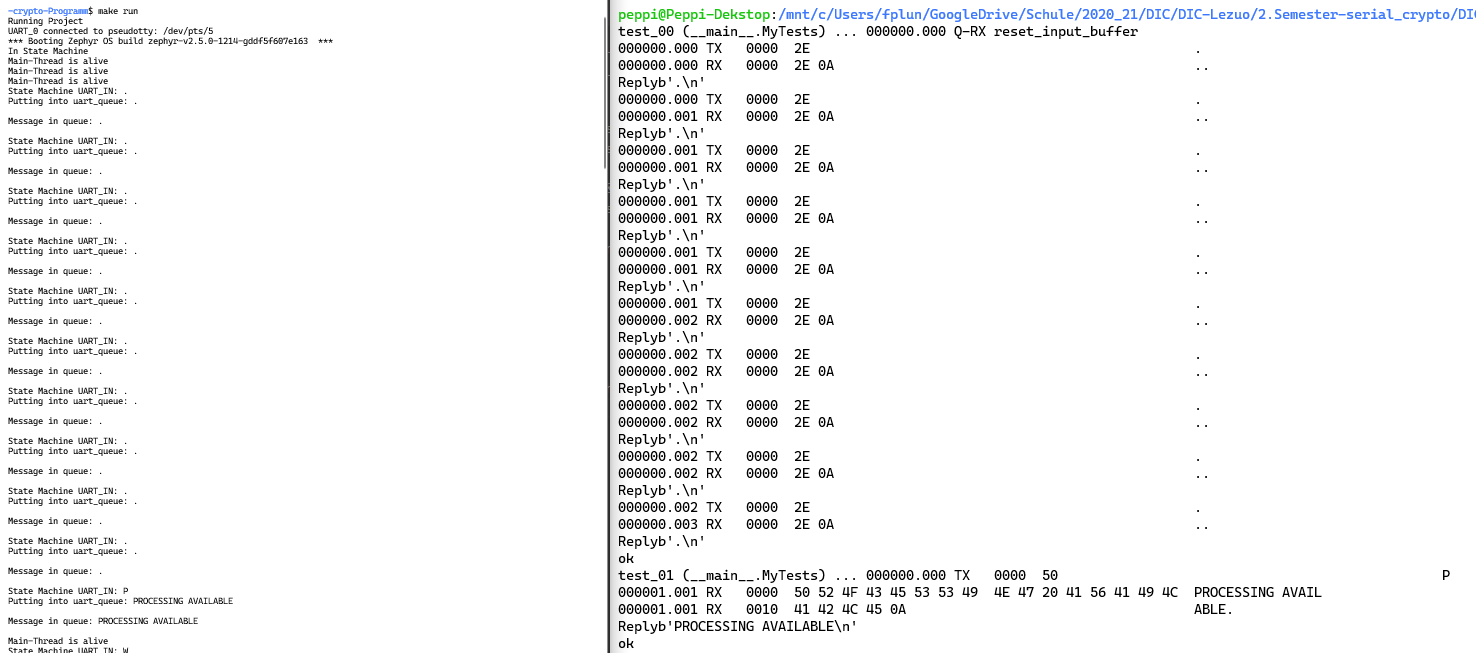
\includegraphics[width=\linewidth]{Test00-01.png}
    \caption{Test00-01}
    \label{caption:Test00-01}
\end{figure}
\begin{figure}[!htb]
    \centering
    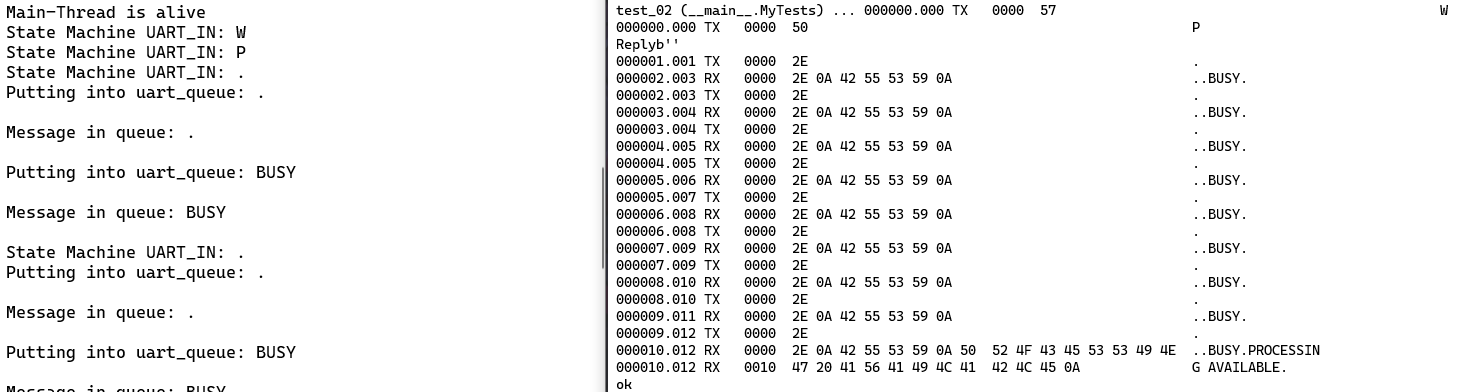
\includegraphics[width=\linewidth]{Test02.png}
    \caption{Test02}
    \label{caption:Test02}
\end{figure}
\begin{figure}[!htb]
    \centering
    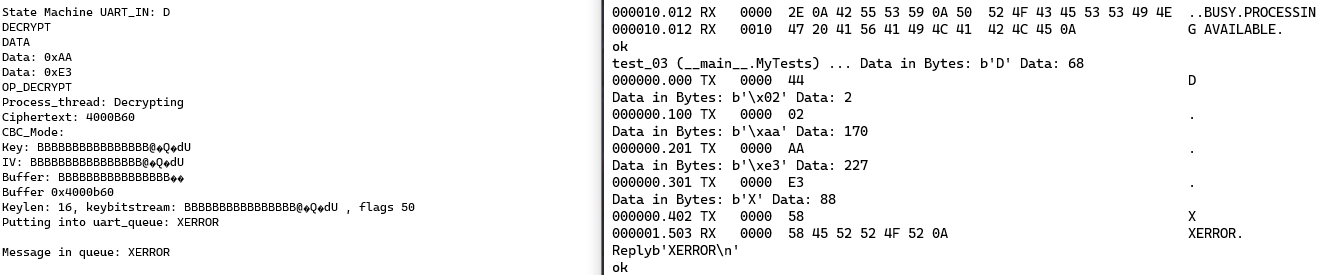
\includegraphics[width=\linewidth]{Test03.png}
    \caption{Test03}
    \label{caption:Test03}
\end{figure}
\begin{figure}[!htb]
    \centering
    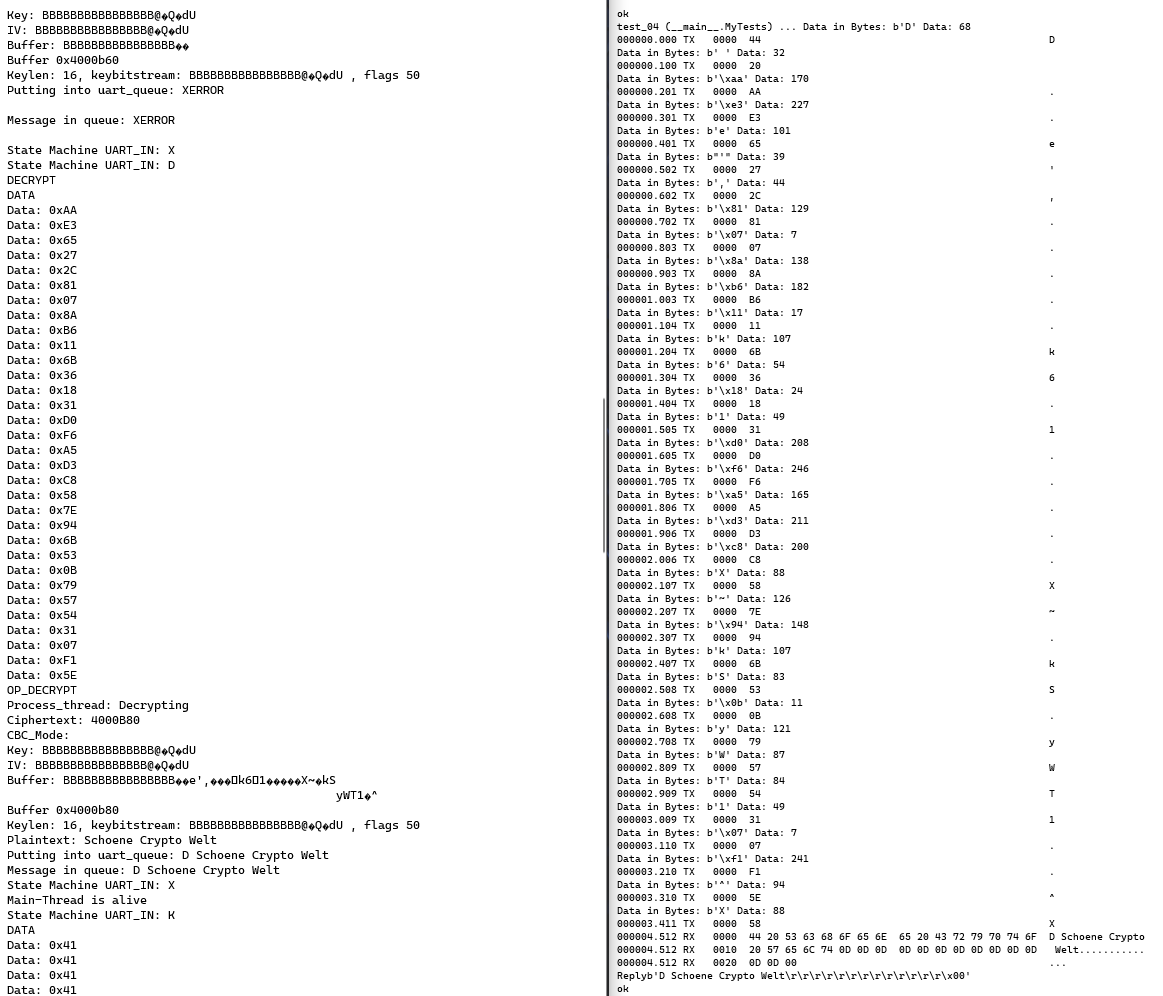
\includegraphics[width=\linewidth]{Test04.png}
    \caption{Test04}
    \label{caption:Test04}
\end{figure}
\begin{figure}[!htb]
    \centering
    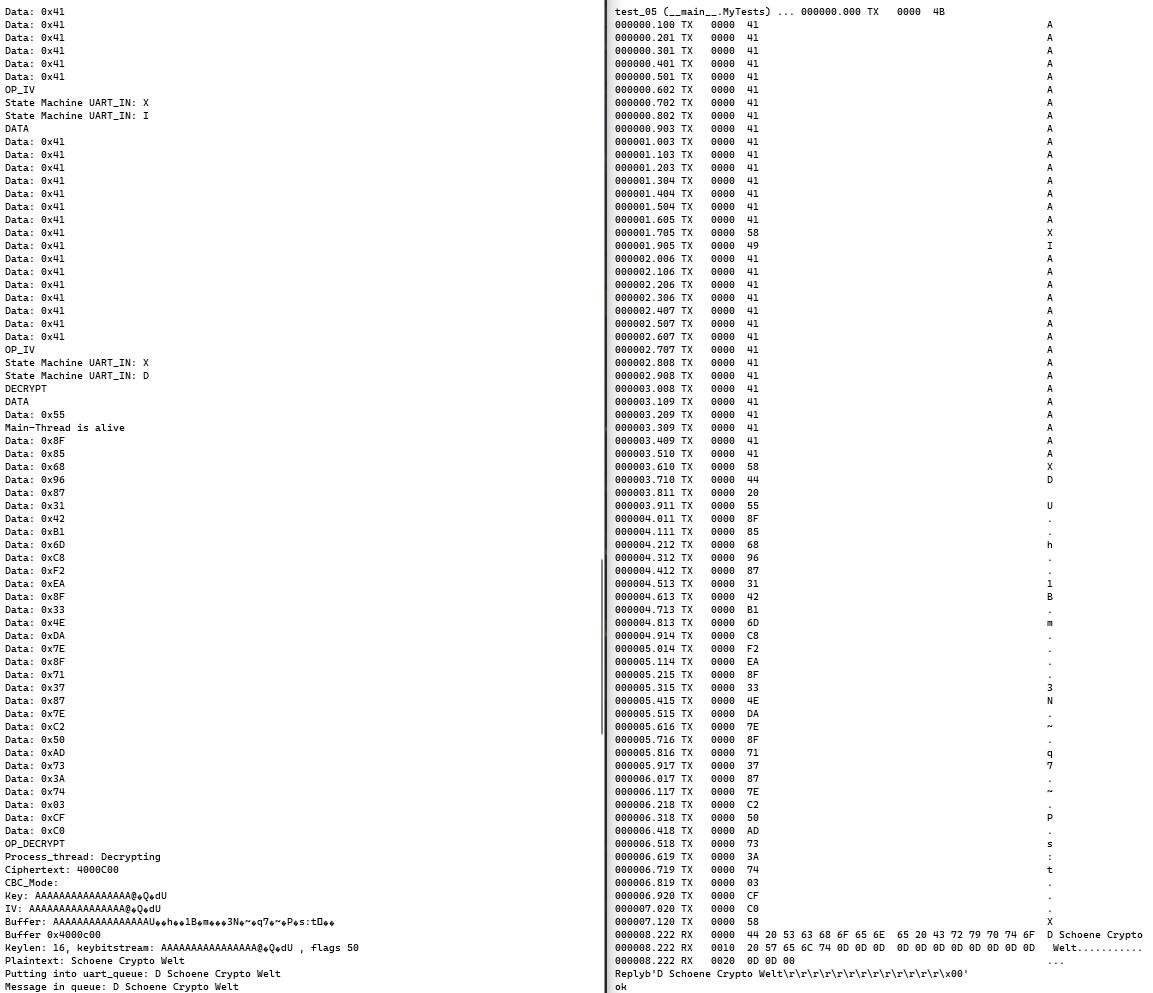
\includegraphics[width=\linewidth]{Test05.png}
    \caption{Test05}
    \label{caption:Test05}
\end{figure}

%-------------------------------------------------------------------------------------------------------
%---------------------------------------------------------------------------------------------------------------------------------------------
%Codeverzeichnis
\end{document}
